% Created by tikzDevice version 0.7.0 on 2014-11-27 09:50:42
% !TEX encoding = UTF-8 Unicode
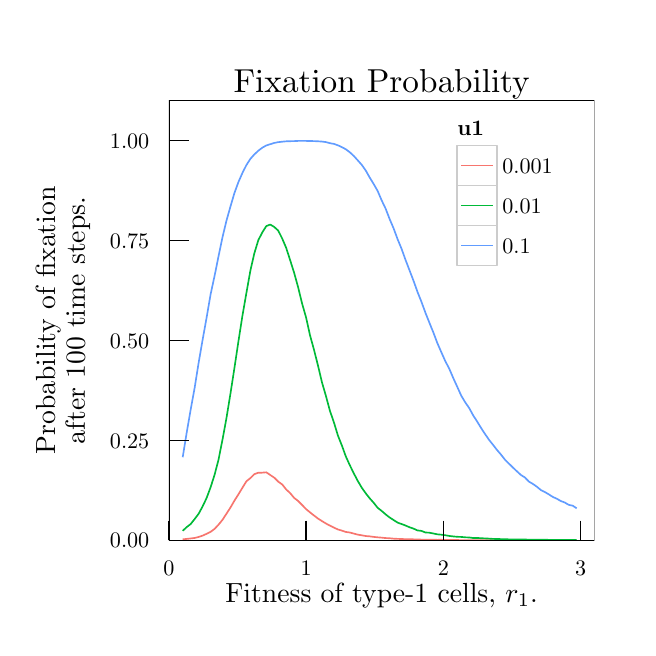
\begin{tikzpicture}[x=1pt,y=1pt]
\definecolor[named]{fillColor}{rgb}{1.00,1.00,1.00}
\path[use as bounding box,fill=fillColor,fill opacity=0.00] (0,0) rectangle (216.81,216.81);
\begin{scope}
\path[clip] (  0.00,  0.00) rectangle (216.81,216.81);
\definecolor[named]{drawColor}{rgb}{1.00,1.00,1.00}
\definecolor[named]{fillColor}{rgb}{1.00,1.00,1.00}

\path[draw=drawColor,line width= 0.6pt,line join=round,line cap=round,fill=fillColor] ( -0.00,  0.00) rectangle (216.81,216.81);
\end{scope}
\begin{scope}
\path[clip] ( 51.06, 31.56) rectangle (204.76,190.48);
\definecolor[named]{fillColor}{rgb}{1.00,1.00,1.00}

\path[fill=fillColor] ( 51.06, 31.56) rectangle (204.76,190.48);
\definecolor[named]{drawColor}{rgb}{0.97,0.46,0.43}

\path[draw=drawColor,line width= 0.6pt,line join=round] ( 56.02, 31.93) --
	( 57.46, 32.07) --
	( 58.90, 32.24) --
	( 60.34, 32.42) --
	( 61.77, 32.78) --
	( 63.21, 33.26) --
	( 64.65, 33.92) --
	( 66.09, 34.63) --
	( 67.53, 35.69) --
	( 68.96, 37.21) --
	( 70.40, 38.98) --
	( 71.84, 41.19) --
	( 73.28, 43.42) --
	( 74.71, 45.90) --
	( 76.15, 48.16) --
	( 77.59, 50.54) --
	( 79.03, 52.89) --
	( 80.47, 54.05) --
	( 81.90, 55.47) --
	( 83.34, 55.99) --
	( 84.78, 56.01) --
	( 86.22, 56.14) --
	( 87.65, 55.17) --
	( 89.09, 54.21) --
	( 90.53, 52.77) --
	( 91.97, 51.76) --
	( 93.41, 49.95) --
	( 94.84, 48.63) --
	( 96.28, 46.90) --
	( 97.72, 45.79) --
	( 99.16, 44.35) --
	(100.60, 42.84) --
	(102.03, 41.66) --
	(103.47, 40.53) --
	(104.91, 39.43) --
	(106.35, 38.51) --
	(107.78, 37.64) --
	(109.22, 36.87) --
	(110.66, 36.15) --
	(112.10, 35.49) --
	(113.54, 35.08) --
	(114.97, 34.59) --
	(116.41, 34.38) --
	(117.85, 34.00) --
	(119.29, 33.61) --
	(120.73, 33.38) --
	(122.16, 33.11) --
	(123.60, 33.00) --
	(125.04, 32.80) --
	(126.48, 32.65) --
	(127.91, 32.53) --
	(129.35, 32.38) --
	(130.79, 32.31) --
	(132.23, 32.16) --
	(133.67, 32.09) --
	(135.10, 32.04) --
	(136.54, 31.98) --
	(137.98, 31.95) --
	(139.42, 31.92) --
	(140.86, 31.87) --
	(142.29, 31.82) --
	(143.73, 31.78) --
	(145.17, 31.75) --
	(146.61, 31.75) --
	(148.04, 31.74) --
	(149.48, 31.75) --
	(150.92, 31.69) --
	(152.36, 31.69) --
	(153.80, 31.66) --
	(155.23, 31.67) --
	(156.67, 31.62) --
	(158.11, 31.63) --
	(159.55, 31.63) --
	(160.99, 31.60) --
	(162.42, 31.62) --
	(163.86, 31.61) --
	(165.30, 31.60) --
	(166.74, 31.60) --
	(168.17, 31.59) --
	(169.61, 31.58) --
	(171.05, 31.59) --
	(172.49, 31.59) --
	(173.93, 31.59) --
	(175.36, 31.58) --
	(176.80, 31.59) --
	(178.24, 31.57) --
	(179.68, 31.57) --
	(181.11, 31.57) --
	(182.55, 31.57) --
	(183.99, 31.58) --
	(185.43, 31.57) --
	(186.87, 31.57) --
	(188.30, 31.57) --
	(189.74, 31.57) --
	(191.18, 31.57) --
	(192.62, 31.56) --
	(194.06, 31.56) --
	(195.49, 31.56) --
	(196.93, 31.56) --
	(198.37, 31.56);
\definecolor[named]{drawColor}{rgb}{0.00,0.73,0.22}

\path[draw=drawColor,line width= 0.6pt,line join=round] ( 56.02, 35.00) --
	( 57.46, 36.33) --
	( 58.90, 37.45) --
	( 60.34, 39.26) --
	( 61.77, 41.15) --
	( 63.21, 43.81) --
	( 64.65, 46.84) --
	( 66.09, 50.71) --
	( 67.53, 55.22) --
	( 68.96, 60.70) --
	( 70.40, 67.94) --
	( 71.84, 75.79) --
	( 73.28, 84.61) --
	( 74.71, 93.83) --
	( 76.15,103.43) --
	( 77.59,112.64) --
	( 79.03,120.91) --
	( 80.47,129.01) --
	( 81.90,135.26) --
	( 83.34,140.02) --
	( 84.78,142.83) --
	( 86.22,145.10) --
	( 87.65,145.67) --
	( 89.09,144.80) --
	( 90.53,143.49) --
	( 91.97,140.62) --
	( 93.41,137.24) --
	( 94.84,132.81) --
	( 96.28,128.25) --
	( 97.72,123.03) --
	( 99.16,117.12) --
	(100.60,112.10) --
	(102.03,105.62) --
	(103.47,100.40) --
	(104.91, 94.69) --
	(106.35, 88.62) --
	(107.78, 83.71) --
	(109.22, 78.36) --
	(110.66, 74.18) --
	(112.10, 69.44) --
	(113.54, 65.82) --
	(114.97, 61.85) --
	(116.41, 58.69) --
	(117.85, 55.76) --
	(119.29, 53.00) --
	(120.73, 50.57) --
	(122.16, 48.55) --
	(123.60, 46.73) --
	(125.04, 45.11) --
	(126.48, 43.30) --
	(127.91, 42.19) --
	(129.35, 40.94) --
	(130.79, 39.81) --
	(132.23, 38.90) --
	(133.67, 37.96) --
	(135.10, 37.45) --
	(136.54, 36.91) --
	(137.98, 36.29) --
	(139.42, 35.79) --
	(140.86, 35.14) --
	(142.29, 34.97) --
	(143.73, 34.39) --
	(145.17, 34.32) --
	(146.61, 34.03) --
	(148.04, 33.73) --
	(149.48, 33.60) --
	(150.92, 33.40) --
	(152.36, 33.14) --
	(153.80, 32.97) --
	(155.23, 32.84) --
	(156.67, 32.79) --
	(158.11, 32.65) --
	(159.55, 32.59) --
	(160.99, 32.40) --
	(162.42, 32.43) --
	(163.86, 32.31) --
	(165.30, 32.26) --
	(166.74, 32.18) --
	(168.17, 32.08) --
	(169.61, 32.05) --
	(171.05, 32.00) --
	(172.49, 32.00) --
	(173.93, 31.90) --
	(175.36, 31.92) --
	(176.80, 31.87) --
	(178.24, 31.89) --
	(179.68, 31.84) --
	(181.11, 31.82) --
	(182.55, 31.79) --
	(183.99, 31.77) --
	(185.43, 31.76) --
	(186.87, 31.78) --
	(188.30, 31.73) --
	(189.74, 31.69) --
	(191.18, 31.71) --
	(192.62, 31.71) --
	(194.06, 31.70) --
	(195.49, 31.71) --
	(196.93, 31.67) --
	(198.37, 31.68);
\definecolor[named]{drawColor}{rgb}{0.38,0.61,1.00}

\path[draw=drawColor,line width= 0.6pt,line join=round] ( 56.02, 61.59) --
	( 57.46, 70.48) --
	( 58.90, 78.80) --
	( 60.34, 86.70) --
	( 61.77, 95.70) --
	( 63.21,104.01) --
	( 64.65,112.01) --
	( 66.09,120.41) --
	( 67.53,127.10) --
	( 68.96,134.19) --
	( 70.40,141.10) --
	( 71.84,147.10) --
	( 73.28,152.20) --
	( 74.71,157.06) --
	( 76.15,161.02) --
	( 77.59,164.28) --
	( 79.03,167.15) --
	( 80.47,169.40) --
	( 81.90,171.00) --
	( 83.34,172.34) --
	( 84.78,173.44) --
	( 86.22,174.24) --
	( 87.65,174.70) --
	( 89.09,175.15) --
	( 90.53,175.44) --
	( 91.97,175.60) --
	( 93.41,175.74) --
	( 94.84,175.79) --
	( 96.28,175.82) --
	( 97.72,175.89) --
	( 99.16,175.89) --
	(100.60,175.89) --
	(102.03,175.85) --
	(103.47,175.82) --
	(104.91,175.75) --
	(106.35,175.65) --
	(107.78,175.46) --
	(109.22,175.07) --
	(110.66,174.81) --
	(112.10,174.30) --
	(113.54,173.64) --
	(114.97,172.86) --
	(116.41,171.78) --
	(117.85,170.45) --
	(119.29,168.85) --
	(120.73,167.23) --
	(122.16,165.19) --
	(123.60,162.64) --
	(125.04,160.30) --
	(126.48,157.77) --
	(127.91,154.41) --
	(129.35,151.40) --
	(130.79,147.66) --
	(132.23,144.28) --
	(133.67,140.38) --
	(135.10,136.91) --
	(136.54,132.88) --
	(137.98,129.13) --
	(139.42,125.36) --
	(140.86,121.33) --
	(142.29,117.73) --
	(143.73,113.80) --
	(145.17,110.17) --
	(146.61,106.62) --
	(148.04,102.81) --
	(149.48, 99.52) --
	(150.92, 96.28) --
	(152.36, 93.54) --
	(153.80, 90.16) --
	(155.23, 87.03) --
	(156.67, 83.83) --
	(158.11, 81.42) --
	(159.55, 79.34) --
	(160.99, 76.69) --
	(162.42, 74.49) --
	(163.86, 72.12) --
	(165.30, 69.94) --
	(166.74, 67.84) --
	(168.17, 66.05) --
	(169.61, 64.19) --
	(171.05, 62.52) --
	(172.49, 60.67) --
	(173.93, 59.25) --
	(175.36, 57.84) --
	(176.80, 56.49) --
	(178.24, 55.17) --
	(179.68, 54.27) --
	(181.11, 52.79) --
	(182.55, 51.94) --
	(183.99, 50.94) --
	(185.43, 49.75) --
	(186.87, 49.02) --
	(188.30, 48.18) --
	(189.74, 47.25) --
	(191.18, 46.61) --
	(192.62, 45.78) --
	(194.06, 45.23) --
	(195.49, 44.39) --
	(196.93, 44.08) --
	(198.37, 43.13);
\definecolor[named]{drawColor}{rgb}{0.00,0.00,0.00}

\path[draw=drawColor,line width= 0.6pt,line join=round,line cap=round] ( 51.06, 31.56) rectangle (204.76,190.48);
\end{scope}
\begin{scope}
\path[clip] (  0.00,  0.00) rectangle (216.81,216.81);
\definecolor[named]{drawColor}{rgb}{0.00,0.00,0.00}

\node[text=drawColor,anchor=base east,inner sep=0pt, outer sep=0pt, scale=  0.80] at ( 43.95, 28.80) {0.00};

\node[text=drawColor,anchor=base east,inner sep=0pt, outer sep=0pt, scale=  0.80] at ( 43.95, 64.92) {0.25};

\node[text=drawColor,anchor=base east,inner sep=0pt, outer sep=0pt, scale=  0.80] at ( 43.95,101.04) {0.50};

\node[text=drawColor,anchor=base east,inner sep=0pt, outer sep=0pt, scale=  0.80] at ( 43.95,137.16) {0.75};

\node[text=drawColor,anchor=base east,inner sep=0pt, outer sep=0pt, scale=  0.80] at ( 43.95,173.28) {1.00};
\end{scope}
\begin{scope}
\path[clip] (  0.00,  0.00) rectangle (216.81,216.81);
\definecolor[named]{drawColor}{rgb}{0.00,0.00,0.00}

\path[draw=drawColor,line width= 0.6pt,line join=round] ( 58.18, 31.56) --
	( 51.06, 31.56);

\path[draw=drawColor,line width= 0.6pt,line join=round] ( 58.18, 67.67) --
	( 51.06, 67.67);

\path[draw=drawColor,line width= 0.6pt,line join=round] ( 58.18,103.79) --
	( 51.06,103.79);

\path[draw=drawColor,line width= 0.6pt,line join=round] ( 58.18,139.91) --
	( 51.06,139.91);

\path[draw=drawColor,line width= 0.6pt,line join=round] ( 58.18,176.03) --
	( 51.06,176.03);
\end{scope}
\begin{scope}
\path[clip] (  0.00,  0.00) rectangle (216.81,216.81);
\definecolor[named]{drawColor}{rgb}{0.00,0.00,0.00}

\path[draw=drawColor,line width= 0.6pt,line join=round] ( 51.06, 38.67) --
	( 51.06, 31.56);

\path[draw=drawColor,line width= 0.6pt,line join=round] (100.65, 38.67) --
	(100.65, 31.56);

\path[draw=drawColor,line width= 0.6pt,line join=round] (150.23, 38.67) --
	(150.23, 31.56);

\path[draw=drawColor,line width= 0.6pt,line join=round] (199.81, 38.67) --
	(199.81, 31.56);
\end{scope}
\begin{scope}
\path[clip] (  0.00,  0.00) rectangle (216.81,216.81);
\definecolor[named]{drawColor}{rgb}{0.00,0.00,0.00}

\node[text=drawColor,anchor=base,inner sep=0pt, outer sep=0pt, scale=  0.80] at ( 51.06, 18.93) {0};

\node[text=drawColor,anchor=base,inner sep=0pt, outer sep=0pt, scale=  0.80] at (100.65, 18.93) {1};

\node[text=drawColor,anchor=base,inner sep=0pt, outer sep=0pt, scale=  0.80] at (150.23, 18.93) {2};

\node[text=drawColor,anchor=base,inner sep=0pt, outer sep=0pt, scale=  0.80] at (199.81, 18.93) {3};
\end{scope}
\begin{scope}
\path[clip] (  0.00,  0.00) rectangle (216.81,216.81);
\definecolor[named]{drawColor}{rgb}{0.00,0.00,0.00}

\node[text=drawColor,anchor=base,inner sep=0pt, outer sep=0pt, scale=  1.00] at (127.91,  9.03) {Fitness of type-1 cells, $r_1$.};
\end{scope}
\begin{scope}
\path[clip] (  0.00,  0.00) rectangle (216.81,216.81);
\definecolor[named]{drawColor}{rgb}{0.00,0.00,0.00}

\node[text=drawColor,rotate= 90.00,anchor=base,inner sep=0pt, outer sep=0pt, scale=  1.00] at (  9.90,111.02) {Probability of fixation };

\node[text=drawColor,rotate= 90.00,anchor=base,inner sep=0pt, outer sep=0pt, scale=  1.00] at ( 20.70,111.02) {  after 100 time steps.};
\end{scope}
\begin{scope}
\path[clip] (  0.00,  0.00) rectangle (216.81,216.81);
\definecolor[named]{fillColor}{rgb}{1.00,1.00,1.00}

\path[fill=fillColor] (150.98,126.59) rectangle (194.00,187.62);
\end{scope}
\begin{scope}
\path[clip] (  0.00,  0.00) rectangle (216.81,216.81);
\definecolor[named]{drawColor}{rgb}{0.00,0.00,0.00}

\node[text=drawColor,anchor=base west,inner sep=0pt, outer sep=0pt, scale=  0.80] at (155.25,177.83) {\bfseries u1};
\end{scope}
\begin{scope}
\path[clip] (  0.00,  0.00) rectangle (216.81,216.81);
\definecolor[named]{drawColor}{rgb}{0.80,0.80,0.80}
\definecolor[named]{fillColor}{rgb}{1.00,1.00,1.00}

\path[draw=drawColor,line width= 0.6pt,line join=round,line cap=round,fill=fillColor] (155.25,159.76) rectangle (169.70,174.22);
\end{scope}
\begin{scope}
\path[clip] (  0.00,  0.00) rectangle (216.81,216.81);
\definecolor[named]{drawColor}{rgb}{0.97,0.46,0.43}

\path[draw=drawColor,line width= 0.6pt,line join=round] (156.69,166.99) -- (168.26,166.99);
\end{scope}
\begin{scope}
\path[clip] (  0.00,  0.00) rectangle (216.81,216.81);
\definecolor[named]{drawColor}{rgb}{0.80,0.80,0.80}
\definecolor[named]{fillColor}{rgb}{1.00,1.00,1.00}

\path[draw=drawColor,line width= 0.6pt,line join=round,line cap=round,fill=fillColor] (155.25,145.31) rectangle (169.70,159.76);
\end{scope}
\begin{scope}
\path[clip] (  0.00,  0.00) rectangle (216.81,216.81);
\definecolor[named]{drawColor}{rgb}{0.00,0.73,0.22}

\path[draw=drawColor,line width= 0.6pt,line join=round] (156.69,152.54) -- (168.26,152.54);
\end{scope}
\begin{scope}
\path[clip] (  0.00,  0.00) rectangle (216.81,216.81);
\definecolor[named]{drawColor}{rgb}{0.80,0.80,0.80}
\definecolor[named]{fillColor}{rgb}{1.00,1.00,1.00}

\path[draw=drawColor,line width= 0.6pt,line join=round,line cap=round,fill=fillColor] (155.25,130.86) rectangle (169.70,145.31);
\end{scope}
\begin{scope}
\path[clip] (  0.00,  0.00) rectangle (216.81,216.81);
\definecolor[named]{drawColor}{rgb}{0.38,0.61,1.00}

\path[draw=drawColor,line width= 0.6pt,line join=round] (156.69,138.08) -- (168.26,138.08);
\end{scope}
\begin{scope}
\path[clip] (  0.00,  0.00) rectangle (216.81,216.81);
\definecolor[named]{drawColor}{rgb}{0.00,0.00,0.00}

\node[text=drawColor,anchor=base west,inner sep=0pt, outer sep=0pt, scale=  0.80] at (171.51,164.24) {0.001};
\end{scope}
\begin{scope}
\path[clip] (  0.00,  0.00) rectangle (216.81,216.81);
\definecolor[named]{drawColor}{rgb}{0.00,0.00,0.00}

\node[text=drawColor,anchor=base west,inner sep=0pt, outer sep=0pt, scale=  0.80] at (171.51,149.78) {0.01};
\end{scope}
\begin{scope}
\path[clip] (  0.00,  0.00) rectangle (216.81,216.81);
\definecolor[named]{drawColor}{rgb}{0.00,0.00,0.00}

\node[text=drawColor,anchor=base west,inner sep=0pt, outer sep=0pt, scale=  0.80] at (171.51,135.33) {0.1};
\end{scope}
\begin{scope}
\path[clip] (  0.00,  0.00) rectangle (216.81,216.81);
\definecolor[named]{drawColor}{rgb}{0.00,0.00,0.00}

\node[text=drawColor,anchor=base,inner sep=0pt, outer sep=0pt, scale=  1.20] at (127.91,193.49) {Fixation Probability};
\end{scope}
\end{tikzpicture}
